% 06.1.6. ESFUERZOS REALES DE LAS TAREAS POR ITERACIÓN 
%----------------------------------------------------------------------------------------

\paragraph{} Para mostrar los esfuerzos reales de cada iteración se han realizado varias gráficas.

\paragraph{} Como se aprecia en la ~\cref{fig:6161} el mes de más trabajo fue Marzo. Además se muestran las horas invertidas en el proyecto y concretamente en cada una de las tareas. En total se realizaron 274 horas frente a las 339 previstas. Pero estas 339 son con la corrección aplicada al desconocimiento de las mismas al inicio del proyecto. Sin esa corrección se estimaron 212 por lo que se han mantenido las horas entre ambas.

\begin{figure}[h!]
\centering
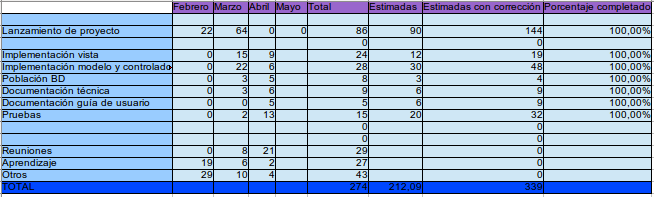
\includegraphics[width=0.95\textwidth]{img/6161}
\caption{Esfuerzos reales primera iteración}
 \label{fig:6161}
\end{figure}

\paragraph{} En la figura ~\cref{fig:6162} se muestra lo anterior más gráficamente. La ultima columna sería el global de la primera iteración y las demás las subtareas.

\begin{figure}[h!]
\centering
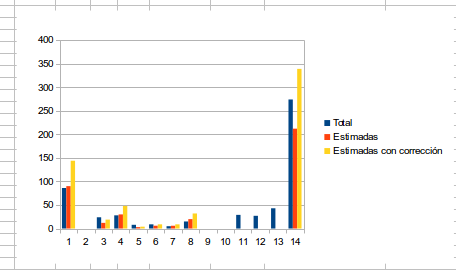
\includegraphics[width=0.85\textwidth]{img/6162}
\caption{Esfuerzos reales primera iteración}
 \label{fig:6162}
\end{figure}


\paragraph{} Para la segunda iteración se muestran la misma gráficas utilizadas para el análisis de la primera iteración pero con las horas invertidas en la segunda iteración (~\cref{fig:6163} y ~\cref{fig:6164}).

\begin{figure}[h!]
\centering
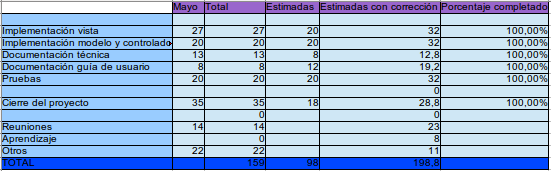
\includegraphics[width=0.95\textwidth]{img/6163}
\caption{Esfuerzos reales segunda iteración}
 \label{fig:6163}
\end{figure}

\begin{figure}[h!]
\centering
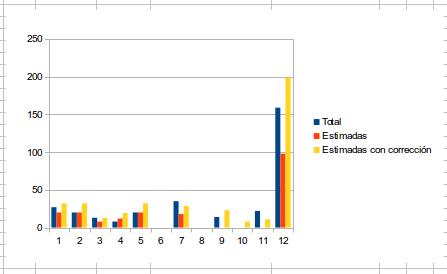
\includegraphics[width=0.95\textwidth]{img/6164}
\caption{Esfuerzos reales segunda iteración}
 \label{fig:6164}
\end{figure}